%%%%%%%%%%%%%%%%%%%%%%%%%%%%%%%%%%%%%%%%%%%%%%%%
%% Compile the master file!
%% 		Slides: Antonio Machicao y Priemer
%% 		Course: Wissenschaftliches Arbeiten
%%%%%%%%%%%%%%%%%%%%%%%%%%%%%%%%%%%%%%%%%%%%%%%%


%%%%%%%%%%%%%%%%%%%%%%%%%%%%%%%%%%%%%%%%%%%%%%%%%%%%
%%%             Metadata                         
%%%%%%%%%%%%%%%%%%%%%%%%%%%%%%%%%%%%%%%%%%%%%%%%%%%%  

\title{
	\LaTeX\ for Linguists
}

\subtitle{\LaTeX\ 7: Math mode 2 \& trees}

\author[aMyP]{
	{\small Sebastian Nordhoff \& Antonio Machicao y Priemer}
	\\
	{\footnotesize \url{www.linguistik.hu-berlin.de/staff/amyp}}
	%	\\
	%	{\footnotesize \href{mailto:mapriema@hu-berlin.de}{mapriema@hu-berlin.de}}
}

\institute{LOT 2019, Amsterdam}

%\date{ }

%\publishers{\textbf{6. linguistischer Methodenworkshop \\ Humboldt-Universität zu Berlin}}

%\hyphenation{nobreak}


%%%%%%%%%%%%%%%%%%%%%%%%%%%%%%%%%%%%%%%%%%%%%%%%%%%%
%%%             Preamble's End                   
%%%%%%%%%%%%%%%%%%%%%%%%%%%%%%%%%%%%%%%%%%%%%%%%%%%%      


%%%%%%%%%%%%%%%%%%%%%%%%%%%%%%%%%%%
%%%%%%%%%%%%%%%%%%%%%%%%%%%%%%%%%%%    
%% Title slide 
\begin{frame}
  \HUtitle
\end{frame}


%% Contents slide
\frame{
%\begin{multicols}{2}
	\frametitle{Contents}
%	\tableofcontents[hideallsubsections]
	\tableofcontents
	%[pausesections]
%\end{multicols}
	}


%%%%%%%%%%%%%%%%%%%%%%%%%%%%%%%%%%%%
%%%%%%%%%%%%%%%%%%%%%%%%%%%%%%%%%%%%
%% Extra literature

\nocite{Freitag&MyP15a}
\nocite{Knuth1986}
\nocite{Kopka94a}
\nocite{MyP17c}
\nocite{MyP&Kerkhof16a}
	
%%%%%%%%%%%%%%%%%%%%%%%%%%%%%%%%%%%%
%%%%%%%%%%%%%%%%%%%%%%%%%%%%%%%%%%%%


%%%%%%%%%%%%%%%%%%%%%%%%%%%%%%%%%%%%%
%%%%%%%%%%%%%%%%%%%%%%%%%%%%%%%%%%%%%
%%%% Basic literature for these slides
%
%\begin{frame}
%\frametitle{Grundlage \& empfohlene Lektüre}
%
%\dots basierend auf \citet{Freitag&MyP15a} und auf \citet{MyP&Kerkhof16a}\\
%\ras \href{https://www.researchgate.net/publication/279514740_LATEX-Einfuhrung_fur_Linguisten}{LINK}
%
%
%\nocite{Kopka94a}
%
%\end{frame}


%%%%%%%%%%%%%%%%%%%%%%%%%%%%%%%%%%
%%%%%%%%%%%%%%%%%%%%%%%%%%%%%%%%%%
\section{Math mode 2}
\frame{
	\frametitle{~}
	\begin{multicols}{2}
		\tableofcontents[currentsection,hideallsubsections]
	\end{multicols}
}
%%%%%%%%%%%%%%%%%%%%%%%%%%%%%%%%%%


%%%%%%%%%%%%%%%%%%%%%%%%%%%%%%%%%%
%%%%%%%%%%%%%%%%%%%%%%%%%%%%%%%%%%
\subsection{Non-exhaustive lists of symbols}
%\frame{
%	\frametitle{~}
%	\begin{multicols}{2}
%		\tableofcontents[currentsection,hideallsubsections]
%	\end{multicols}
%}
%%%%%%%%%%%%%%%%%%%%%%%%%%%%%%%%%%

\begin{frame}[fragile]
\frametitle{Non-exhaustive lists of symbols}

Symbols you could need (the following lists are by no means exhaustive):

\begin{table}
	\centering
	\scalebox{.9}{
		\begin{tabular}{ll|ll|ll}
			$=$ & \texttt{=} & $\sim$ & \texttt{\textbackslash sim} & $\infty$ & \texttt{\textbackslash infty} \\
			$\pm$	&	\texttt{\textbackslash pm}	&$\approx$	&	\texttt{\textbackslash approx}	&$\emptyset$	&	\texttt{\textbackslash emptyset}	\\
			$\cdot$	&	\texttt{\textbackslash cdot}	&$\subset$	&	\texttt{\textbackslash subset}	&$\Box$	&	\texttt{\textbackslash Box}	\\
			$\times$	&	\texttt{\textbackslash times}	&$\supset$	&	\texttt{\textbackslash supset}	&$\%$	&	\texttt{\textbackslash \%}	\\
			$\circ$	&	\texttt{\textbackslash circ}	&$\subseteq$	&	\texttt{\textbackslash subseteq}	&$\$$	&	\texttt{\textbackslash $\$$}	\\
			$\in$	&	\texttt{\textbackslash in}	&$\cap$	&	\texttt{\textbackslash cap}		&$\&$	&	\texttt{\textbackslash $\&$}	\\
			$\ni$	&	\texttt{\textbackslash ni}	&$\cup$	&	\texttt{\textbackslash cup}		&$\#$	&	\texttt{\textbackslash $\#$}	\\
			$\neq$	&	\texttt{\textbackslash neq}	&$\forall$	&	\texttt{\textbackslash forall}	&$\backslash$	&	\texttt{\textbackslash backslash}	\\
			$\leq$	&	\texttt{\textbackslash leq}	&$\exists$	&	\texttt{\textbackslash exists}	&$\dots$		&	\texttt{\textbackslash dots}	\\
			$\geq$	&	\texttt{\textbackslash geq}	&$\land$	&	\texttt{\textbackslash land}	&$<$	&	\texttt{$<$}	\\
			$\ll$	&	\texttt{\textbackslash ll}	&$\lor$		&	\texttt{\textbackslash lor}	&$>$	&	\texttt{$>$}	\\
			$\gg$	&	\texttt{\textbackslash gg}	&$\lnot$	&	\texttt{\textbackslash lnot}	&	&	\\
		\end{tabular}
	}
	\caption{Some non-specific symbols}
\end{table}

%\hfill \dots\ not an exhaustive list.

\end{frame}


%%%%%%%%%%%%%%%%%%%%%%%%%%%%%%%%%%
\begin{frame}
%\frametitle{(Einige) Zeichen im Mathematikmodus}

\begin{table}

	\centering
	\scalebox{.8}{
		\begin{tabular}{llllll}
			$\rightarrow$	&	\texttt{\textbackslash rightarrow}	&$\Downarrow$	&	\texttt{\textbackslash Downarrow}	&$\{\}$	&	\texttt{\textbackslash\{\textbackslash\}}	\\
			$\leftarrow$	&	\texttt{\textbackslash leftarrow}	&$\mapsto$	&	\texttt{\textbackslash mapsto}	&$\mathcal{A}$	&	\texttt{\textbackslash mathcal\{A\}}	\\
			$\leftrightarrow$	&	\texttt{\textbackslash leftrightarrow}	&$\leadsto$	&	\texttt{\textbackslash leadsto}	&$\mathfrak{A}$	&	\texttt{\textbackslash mathfrak\{A\}}	\\
			$\Rightarrow$	&	\texttt{\textbackslash Rightarrow}	&$\xrightarrow[abc]{xyz}$	&	\texttt{\textbackslash xrightarrow[abc]\{xyz\}}	&$\mathbb{R}$	&	\texttt{\textbackslash mathbb\{R\}}	\\
			$\Leftarrow$	&	\texttt{\textbackslash Leftarrow}	&$()$	&	\texttt{()}	&$\aleph$	&	\texttt{\textbackslash aleph}	\\
			$\Leftrightarrow$	&	\texttt{\textbackslash Leftrightarrow}	&$[]$	&\texttt{[]}	&	&	\\
		\end{tabular}
	}
	\caption{Some arrows, brackets, fonts}
\end{table}

%\hfill \dots\ not an exhaustive list.
%
%\end{frame}
%
%
%%%%%%%%%%%%%%%%%%%%%%%%%%%%%%%%%%%
%\begin{frame}\frametitle{(Einige) Zeichen im Mathematikmodus}

\begin{table}

\centering
%\scalebox{.8}{
\begin{tabular}{ll|ll|ll}
	$\alpha$ &	\texttt{\textbackslash alpha}	&$\theta$	&	\texttt{\textbackslash theta}	&$\varepsilon$	&	\texttt{\textbackslash varepsilon}	\\
	$\gamma$&	\texttt{\textbackslash gamma}	&$\phi$	&	\texttt{\textbackslash phi}	&$\vartheta$	&	\texttt{\textbackslash vartheta}	\\
	$\delta$&	\texttt{\textbackslash delta}	&$\Gamma$	&	\texttt{\textbackslash Gamma}	&$\Phi$	&	\texttt{\textbackslash Phi}	\\
	$\epsilon$&	\texttt{\textbackslash epsilon}	&$\Delta$	&	\texttt{\textbackslash Delta}	&$\varphi$	&	\texttt{\textbackslash varphi}	\\
\end{tabular}
%}
\caption{Some Greek letters and variants}
\end{table}

%\hfill \dots\ keine exhaustive Liste

\end{frame}


%%%%%%%%%%%%%%%%%%%%%%%%%%%%%%%%%%
\begin{frame}
%\frametitle{(Einige) Zeichen im Mathematikmodus}

\begin{table}

\centering
%\scalebox{.8}{
\begin{tabular}{ll|ll|ll}

$\tilde{a}$&	\texttt{\textbackslash tilde\{a\}}	&$\notin$	&	\texttt{\textbackslash notin}	&$\widetilde{abc}$	&	\texttt{\textbackslash widetilde\{abc\}}	\\
$\bar{a}$ &	\texttt{\textbackslash bar\{a\}}	&$\dot{a}$	&	\texttt{\textbackslash dot\{a\}}	&$\overline{abc}$	&	\texttt{\textbackslash overline\{abc\}}	\\
$\vec{a}$&	\texttt{\textbackslash vec\{a\}}	&$\ddot{a}$	&	\texttt{\textbackslash ddot\{a\}}	&$\overrightarrow{abc}$	&	\texttt{\textbackslash overrightarrow\{abc\}}	\\
$\hat{a}$&	\texttt{\textbackslash hat\{a\}}	&$\dot{=}$	&	\texttt{\textbackslash ddot\{=\}}	&$\widehat{abc}$	&	\texttt{\textbackslash widehat\{\}}
\end{tabular}
%} 
\caption{Some combinations of symbols}
\end{table}

%\hfill \dots\ keine exhaustive Liste

\end{frame}


%%%%%%%%%%%%%%%%%%%%%%%%%%%%%%%%%%
\begin{frame}

Some lists of symbols for \LaTeX :

\begin{itemize}
\item List of logic symbols (Wikipedia): 

\url{https://en.wikipedia.org/wiki/List_of_logic_symbols}

\item \LaTeX\ for Logicians:

\url{http://www.logicmatters.net/latex-for-logicians/}

\item The Great, Big List of \LaTeX\ Symbols: \citet{Carlisle&Co01a}

\item The Comprehensive \LaTeX\ Symbol List -- Symbols accessible from \LaTeX :  \citet{Pakin17a}
\end{itemize}

\bigskip

Draw the symbol and get the code:

\begin{itemize}
\item \url{http://detexify.kirelabs.org}
\end{itemize}
\end{frame}


%%%%%%%%%%%%%%%%%%%%%%%%%%%%%%%%%%%
%%%%%%%%%%%%%%%%%%%%%%%%%%%%%%%%%%%
%\subsection{Examples}
%\frame{
%	\frametitle{~}
%	\begin{multicols}{2}
%		\tableofcontents[currentsection,hideallsubsections]
%	\end{multicols}
%}
%%%%%%%%%%%%%%%%%%%%%%%%%%%%%%%%%%%
%%%%%%%%%%%%%%%%%%%%%%%%%%%%%%%%%%%

%%%%%%%%%%%%%%%%%%%%%%%%%%%%%%%%%%
%%%%%%%%%%%%%%%%%%%%%%%%%%%%%%%%%%
\subsection{Example: Set theory}
%\frame{
%	\frametitle{~}
%	\begin{multicols}{2}
%		\tableofcontents[currentsection,hideallsubsections]
%	\end{multicols}
%}
%%%%%%%%%%%%%%%%%%%%%%%%%%%%%%%%%%
%%%%%%%%%%%%%%%%%%%%%%%%%%%%%%%%%%

\begin{frame}[fragile]
\frametitle{Set theory}


{\small
\begin{lstlisting}
$\{\textrm{a}\} \subset \{\textrm{a, e}\}$
\end{lstlisting}
}

\ea $\{\textrm{a}\} \subset \{\textrm{a, e}\}$
\z 


{\small
\begin{lstlisting}
$\emptyset \subseteq \{\textrm{a, b}\}$
\end{lstlisting}
}

\ea $\emptyset \subseteq \{\textrm{a, b}\}$
\z 


{\small
\begin{lstlisting}
$\# \{\emptyset, \textrm{a} \} = 2$
\end{lstlisting}
}

\ea $\# \{\emptyset, \textrm{a} \} = 2$
\z 


{\small
\begin{lstlisting}
$\emptyset \in \{\emptyset, \textrm{a} \}$
\end{lstlisting}
}

\ea $\emptyset \in \{\emptyset, \textrm{a} \}$
\z 
\end{frame}


%%%%%%%%%%%%%%%%%%%%%%%%%%%%%%%%%%
\begin{frame}[fragile]

{\small
\begin{lstlisting}
$\emptyset \notin \{\textrm{a}\}$
\end{lstlisting}
}

\ea $\emptyset \notin \{\textrm{a}\}$
\z 


{\small
\begin{lstlisting}
If $|\textrm{A}| = n$ then $|\mathfrak{P}(\textrm{A})|=2^{n}$
\end{lstlisting}
}

\ea If $|\textrm{A}| = n$ then $|\mathfrak{P}(\textrm{A})|=2^{n}$
\z 


{\small
\begin{lstlisting}
$\{\textrm{a, e}\} \setminus \{\textrm{e, u}\} = \{\textrm{a}\}$
\end{lstlisting}
}

\ea $\{\textrm{a, e}\} \setminus \{\textrm{e, u}\} = \{\textrm{a}\}$
\z 

{\small
\begin{lstlisting}
$ \overline{[ \textrm{A} \cup \textrm{B} ]} = 
[ \overline{\textrm{A}} \cap \overline{\textrm{B}} ] $
\end{lstlisting}
}

\ea DeMorgan:
$ \overline{[ \textrm{A} \cup \textrm{B} ]} = 
[ \overline{\textrm{A}} \cap \overline{\textrm{B}} ] $
\z 


\end{frame}


%%%%%%%%%%%%%%%%%%%%%%%%%%%%%%%%%%
%%%%%%%%%%%%%%%%%%%%%%%%%%%%%%%%%%
\subsection{Example: Propositional Logic}
%\frame{
%\frametitle{~}
%\begin{multicols}{2}
%\tableofcontents[currentsection,hideallsubsections]
%\end{multicols}
%}
%%%%%%%%%%%%%%%%%%%%%%%%%%%%%%%%%%
%%%%%%%%%%%%%%%%%%%%%%%%%%%%%%%%%%

\begin{frame}[fragile]
\frametitle{Propositional Logic}

{\small
\begin{lstlisting}
DeMorgan's law:
$\lnot (P \lor Q ) \Leftrightarrow 
(\lnot P \wedge \lnot Q)$

Biconditional law:
$(P \leftrightarrow P) \Leftrightarrow 
((P \rightarrow Q) \wedge (Q \rightarrow P))$

Logical consequence:
$((p \rightarrow q) \wedge p) \Rightarrow q$
\end{lstlisting}
}

\pause 

\ea DeMorgan's law:
$\lnot (P \lor Q ) \Leftrightarrow 
(\lnot P \wedge \lnot Q)$

\ex Biconditional law:
$(P \leftrightarrow P) \Leftrightarrow 
((P \rightarrow Q) \wedge (Q \rightarrow P))$

\ex Logical consequence:
$((p \rightarrow q) \wedge p) \Rightarrow q$

\z 

\end{frame}


%%%%%%%%%%%%%%%%%%%%%%%%%%%%%%%%%%
%%%%%%%%%%%%%%%%%%%%%%%%%%%%%%%%%%
\subsection{Example: Quantifiers}
%\frame{
%\frametitle{~}
%\begin{multicols}{2}
%\tableofcontents[currentsection,hideallsubsections]
%\end{multicols}
%}
%%%%%%%%%%%%%%%%%%%%%%%%%%%%%%%%%%
%%%%%%%%%%%%%%%%%%%%%%%%%%%%%%%%%%

\begin{frame}[fragile]
\frametitle{Quantifiers}

{\small
\begin{lstlisting}
$\exists x [$\textsc{woman}$(x)$ $\land$ \textsc{sleep}$(x)]$ 

$\forall x [$\textsc{woman}$(x)$ $\rightarrow$ \textsc{sleep}$(x)]$
\end{lstlisting}
}


\pause 


\ea \textbf{Existential quantifier:} \emph{A woman sleeps.}

%\alert{
	$\exists x [$\textsc{woman}$(x)$ $\land$ \textsc{sleep}$(x)]$ 
%}

%`Es gibt ein $x$, $x$ ist eine Frau und $x$ schläft.'

$\nrightarrow$ There is only one sleeper.	 


\pause 


\ex \textbf{Allquantor:} \emph{Every woman sleeps.}

%\alert{
	$\forall x [$\textsc{woman}$(x)$ $\rightarrow$ \textsc{sleep}$(x)]$
%}

%\gq{Für alle $x$ gilt, wenn $x$ eine Frau ist dann, schläft $x$.}

$\nrightarrow$ Only women are sleepers. 
\z 

\end{frame}


%%%%%%%%%%%%%%%%%%%%%%%%%%%%%%%%%%
%%%%%%%%%%%%%%%%%%%%%%%%%%%%%%%%%%
\subsection{Meaning brackets}
%\frame{
%\frametitle{~}
%\begin{multicols}{2}
%\tableofcontents[currentsection,hideallsubsections]
%\end{multicols}
%}
%%%%%%%%%%%%%%%%%%%%%%%%%%%%%%%%%%
%%%%%%%%%%%%%%%%%%%%%%%%%%%%%%%%%%

\begin{frame}[fragile]
\frametitle{Meaning brackets}

In order to use the meaning brackets $\lsem \rsem$ you can 

\begin{enumerate}
	\item (using Xe\LaTeX ) copy the Unicode symbol,
	
	\item make an own command for the symbol to use the Unicode symbol,
	
	\item use the package  \ltxpack{MnSymbol}. It provides the meaning brackets a.o.\ symbols.
\end{enumerate}


\begin{lstlisting}
\usepackage{MnSymbol} 
\end{lstlisting}

\bigskip

Meaning brackets can be used \textbf{only in math mode}:

\begin{lstlisting}
$\lsem \alpha \beta \rsem = \lsem \beta \rsem (\lsem \alpha \rsem)$
\end{lstlisting}

\ea $\lsem \alpha \beta \rsem = \lsem \beta \rsem (\lsem \alpha \rsem)$ \hfill [Function application]
\z 

\end{frame}


%%%%%%%%%%%%%%%%%%%%%%%%%%%%%%%%%%
%%%%%%%%%%%%%%%%%%%%%%%%%%%%%%%%%%
\subsection{Writing formulae}
%\frame{
%\frametitle{~}
%\begin{multicols}{2}
%\tableofcontents[currentsection,hideallsubsections]
%\end{multicols}
%}
%%%%%%%%%%%%%%%%%%%%%%%%%%%%%%%%%%
%%%%%%%%%%%%%%%%%%%%%%%%%%%%%%%%%%

\begin{frame}[fragile]
\frametitle{Writing formulae}

\begin{lstlisting}
\ea $\lsem [_{\textrm{PP}}$\emph{in Amsterdam}$] \rsem (s') 
    = \lambda P \lambda x [P(x) \land [x \textrm{ is in Amsterdam in } s']]$
\z 
\end{lstlisting}


\ea $\lsem [_{\textrm{PP}}$\emph{in Amsterdam}$] \rsem (s') = \lambda P \lambda x [P(x) \land [x \textrm{ is in Amsterdam in } s']]$
\z 

\begin{itemize}
	\item \emph{in Amsterdam}: object language
	\item $s', x, P$: variables
	\item \textrm{is in Amsterdam}: invariable predicate
	\item \textrm{PP}: Index
\end{itemize}

\end{frame}


%%%%%%%%%%%%%%%%%%%%%%%%%%%%%%%%%%
%%%%%%%%%%%%%%%%%%%%%%%%%%%%%%%%%%
\section{Trees}
\frame{
	\frametitle{~}
	\begin{multicols}{2}
		\tableofcontents[currentsection,hideallsubsections]
	\end{multicols}
}
%%%%%%%%%%%%%%%%%%%%%%%%%%%%%%%%%%
%%%%%%%%%%%%%%%%%%%%%%%%%%%%%%%%%%

\begin{frame}[fragile]
\frametitle{Trees}

There are different packages for drawing trees:

\begin{itemize}
	\item \ltxpack{qtree}
	\item \ltxpack{pstrees} (anspruchsvollere Syntax, aber mächtiger als \ltxpack{qtree})
	\item \ltxpack{tikz-qtree}
	\item \alert{\ltxpack{forest}} (einfache Syntax, mächtiger als \ltxpack{pstrees} und \ltxpack{qtree}, based on \ltxpack{tikz})
	\item \dots 
\end{itemize}

%Wir werden hier mit \ltxpack{forest} arbeiten, für eine kurze Beschreibung der anderen Pakete siehe \citet{Freitag&MyP15a} oder \citet{Linke05a}.
\end{frame}


%%%%%%%%%%%%%%%%%%%%%%%%%%%%%%%%%%
%%%%%%%%%%%%%%%%%%%%%%%%%%%%%%%%%%
\subsection{Loading forest}
%\frame{
%	\frametitle{~}
%	\begin{multicols}{2}
%		\tableofcontents[currentsection,hideallsubsections]
%	\end{multicols}
%}
%%%%%%%%%%%%%%%%%%%%%%%%%%%%%%%%%%
%%%%%%%%%%%%%%%%%%%%%%%%%%%%%%%%%%

\begin{frame}[fragile]
\frametitle{Loading forest}


\begin{lstlisting}
\usepackage{forest}
\end{lstlisting}

\ltxpack{forest} provides many features for trees needed in linguistics. 

These features can be loaded specifying the option \ltxterm{linguistics}

\begin{lstlisting}
\usepackage[linguistics]{forest}
\end{lstlisting}

%\end{frame}
%
%
%%%%%%%%%%%%%%%%%%%%%%%%%%%%%%%%%%%
%\begin{frame}[fragile]
%%\frametitle{Baumstrukturen}

\begin{minipage}[b]{.48\textwidth}
\begin{figure}
	\centering
	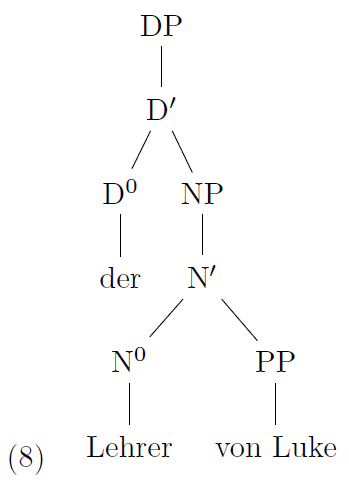
\includegraphics[width=.4\linewidth]{../../texfiles-beamer/tex-material/WissArb-latex/forest2}	
	\caption{without \ltxterm{linguistics}}
\end{figure}
\end{minipage}
%%
%%
\begin{minipage}[b]{.48\textwidth}
\begin{figure}
	\centering
	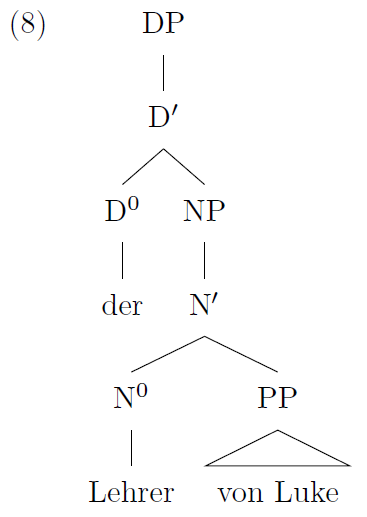
\includegraphics[width=.43\linewidth]{../../texfiles-beamer/tex-material/WissArb-latex/forest1}
	\caption{with \ltxterm{linguistics}}	
\end{figure}
\end{minipage}

\end{frame}


%%%%%%%%%%%%%%%%%%%%%%%%%%%%%%%%%%
\begin{frame}[fragile]
%\frametitle{Baumstrukturen}

\ltxpack{gb4e} re-defines some commands needed for \ltxpack{forest}. If you are using \ltxpack{gb4e}, you must load  \alert{\ltxpack{forest} first} and \alert{\ltxpack{gb4e} after}.

\begin{lstlisting}
\usepackage[linguistics]{forest}

\usepackage{gb4e}
\end{lstlisting}

\end{frame}


%%%%%%%%%%%%%%%%%%%%%%%%%%%%%%%%%%
%%%%%%%%%%%%%%%%%%%%%%%%%%%%%%%%%%
\subsection{forest syntax}
%\frame{
%	\frametitle{~}
%	\begin{multicols}{2}
%		\tableofcontents[currentsection,hideallsubsections]
%	\end{multicols}
%}
%%%%%%%%%%%%%%%%%%%%%%%%%%%%%%%%%%
%%%%%%%%%%%%%%%%%%%%%%%%%%%%%%%%%%

\begin{frame}[fragile]
\frametitle{forest syntax}

\begin{enumerate}
\item Use the \ltxterm{forest} \textbf{environment}.

\item Inside the \ltxterm{forest} environment write the \textbf{bracket notation} for your tree.

\item Do \textbf{not} use \textbf{empty lines}!
\end{enumerate}


\begin{lstlisting}
\begin{forest}
[S [NP] [VP]]
\end{forest}
\end{lstlisting}

\ea \begin{forest}
[S [NP] [VP]]
\end{forest}
\z 

\bigskip 

\begin{itemize}
	\item Practice the bracket notation: \url{http://ironcreek.net/phpsyntaxtree/}
\end{itemize}

\end{frame}


%%%%%%%%%%%%%%%%%%%%%%%%%%%%%%%%%%
\begin{frame}[fragile]
%\frametitle{Baumstrukturen}

For bigger trees, it is useful -- for the sake of clarity -- not to write the bracket notation linearly.

\begin{minipage}[t]{.48\textwidth}
\small	
\begin{lstlisting}
\begin{forest}
[S 
  [NP] 
  [VP
    [NP]
    [V$^{0}$]
  ]
]
\end{forest}
\end{lstlisting}

\vs

\begin{lstlisting}
\begin{forest}
[S [NP] [VP [NP] [V$^{0}$]]]
\end{forest}
\end{lstlisting}
\end{minipage}
%%
%%
\begin{minipage}[t]{.48\textwidth}
\begin{figure}

\centering
\begin{forest}
	[S 
	[NP] 
	[VP
	[NP]
	[V$^{0}$]
	]
	]
\end{forest}

\end{figure}

\end{minipage}

\end{frame}


%%%%%%%%%%%%%%%%%%%%%%%%%%%%%%%%%%
%%%%%%%%%%%%%%%%%%%%%%%%%%%%%%%%%%
\subsection{Trees in example environments}
%\frame{
%	\frametitle{~}
%	\begin{multicols}{2}
%		\tableofcontents[currentsection,hideallsubsections]
%	\end{multicols}
%}
%%%%%%%%%%%%%%%%%%%%%%%%%%%%%%%%%%
%%%%%%%%%%%%%%%%%%%%%%%%%%%%%%%%%%

\begin{frame}[fragile]
\frametitle{Trees in example environments}

\textbf{When using the option \ltxterm{linguistics}}, you can embed the tree in an example environment.


\begin{lstlisting}
\ea 
\begin{forest}
[S [NP] [VP]]
\end{forest}
\z
\end{lstlisting}

\ea 
\begin{forest}
	[S [NP] [VP]]
\end{forest}
\z 

\end{frame}


%%%%%%%%%%%%%%%%%%%%%%%%%%%%%%%%%%
%%%%%%%%%%%%%%%%%%%%%%%%%%%%%%%%%%
\subsection{Abbreviating nodes}
%\frame{
%	\frametitle{~}
%	\begin{multicols}{2}
%		\tableofcontents[currentsection,hideallsubsections]
%	\end{multicols}
%}
%%%%%%%%%%%%%%%%%%%%%%%%%%%%%%%%%%
%%%%%%%%%%%%%%%%%%%%%%%%%%%%%%%%%%

\begin{frame}[fragile]
\frametitle{Abbreviating nodes}


With the option \lstinline|roof|, you can abbreviate nodes.

\begin{multicols}{2}
	
\begin{lstlisting}
\ea 
\begin{forest}
[S 
  [NP [Colourless green ideas, roof]] 
  [VP [sleep furiously, roof]]
]
\end{forest}
\z 
\end{lstlisting}

\ea %
{\scriptsize %
\begin{forest}
	[S [NP [Colourless green ideas, roof]] [VP [sleep furiously, roof]]]
\end{forest}
}
\z 

\end{multicols}

\pause 

Take into account that options in \ltxpack{forest} (based on \ltxterm{TikZ}) are given by a \textbf{comma}. That means, you can use commas only when you \textbf{protect} them.

\begin{multicols}{2}
	
\begin{lstlisting}
\ea 
\begin{forest}
[S [NP [Noam{,} Irene{,} and Angelika, roof]] [VP [sleep, roof]]]
\end{forest}
\z 
\end{lstlisting}
	
	
\ea %
{\scriptsize %
	\begin{forest}
		[S 
		[NP [Noam{,} Irene{,} and Angelika, roof]] 
		[VP [sleep, roof]]
		]
	\end{forest}
}
\z 
\end{multicols}

\end{frame}


%%%%%%%%%%%%%%%%%%%%%%%%%%%%%%%%%%
%%%%%%%%%%%%%%%%%%%%%%%%%%%%%%%%%%
\subsection{Glossing or translating}
%\frame{
%	\frametitle{~}
%	\begin{multicols}{2}
%		\tableofcontents[currentsection,hideallsubsections]
%	\end{multicols}
%}
%%%%%%%%%%%%%%%%%%%%%%%%%%%%%%%%%%
%%%%%%%%%%%%%%%%%%%%%%%%%%%%%%%%%%

\begin{frame}[fragile]
\frametitle{Glossing or translating}


With \lstinline|\\|, you can add \textbf{glosses or translations} to your tree.


\begin{minipage}[t]{.48\textwidth}
\small	
\begin{lstlisting}
\begin{forest}
[S 
  [NP 
    [Peter \\ Peter \\ Pedro, roof]
  ] 
  [VP 
    [schläft tief. \\ sleeps deeply. \\ duerme profundamente, roof]
  ]
]
\end{forest}
\end{lstlisting}
\end{minipage}
%%
%%
\begin{minipage}[t]{.48\textwidth}

\begin{exe}
\ex 
\begin{forest}
[S [NP [Peter \\ Peter \\ Pedro, roof]] 
[VP [schläft tief. \\ 
sleeps deeply. \\ 
duerme profundamente, roof]]]
\end{forest}
\end{exe}
\end{minipage}

\end{frame}


%%%%%%%%%%%%%%%%%%%%%%%%%%%%%%%%%%
%%%%%%%%%%%%%%%%%%%%%%%%%%%%%%%%%%
\subsection{Sub- and superscript}
%\frame{
%	\frametitle{~}
%	\begin{multicols}{2}
%		\tableofcontents[currentsection,hideallsubsections]
%	\end{multicols}
%}
%%%%%%%%%%%%%%%%%%%%%%%%%%%%%%%%%%
%%%%%%%%%%%%%%%%%%%%%%%%%%%%%%%%%%

\begin{frame}[fragile]
\frametitle{Sub- and superscript}

The characters \lstinline|^| and \lstinline|_| are used in \textbf{math mode} for sub- and superscript, respectively. 
	
\begin{multicols}{2}

\begin{lstlisting}
$x^1$

$x_1$
\end{lstlisting}	

\ea $x^1$
\ex $x_1$
\z 

\end{multicols}

\pause 

The \textbf{default scope} of \lstinline|^| and \lstinline|_| is only one character (\ref{ex:SubSup1}), use \lstinline|{ }| to \textbf{expand} it, siehe (\ref{ex:SubSup2}). 


\begin{lstlisting}
\ea X$^1$ Y$^21$ X$_1$ Y$_21$ \label{ex:SubSup1}

\ex X$^{1}$ Y$^{21}$ X$_{1}$ Y$_{21}$ \label{ex:SubSup2}
\z 
\end{lstlisting}


\ea X$^1$ Y$^21$ X$_1$ Y$_21$ \label{ex:SubSup1}

\ex X$^{1}$ Y$^{21}$ X$_{1}$ Y$_{21}$ \label{ex:SubSup2}
\z 

\end{frame}


%%%%%%%%%%%%%%%%%%%%%%%%%%%%%%%%%%%
%\begin{frame}[fragile]
%%\frametitle{Baumstrukturen}
%
%\begin{itemize}
%\item Wie (\ref{ex:BspHochTief}) und (\ref{ex:BspKlammer}) zeigen, verhält sich \textbf{Text innerhalb vom Mathematikmodus} anders (kursiv ohne Spatien). 
%
%\item Um Text wiederzugeben verwenden Sie den Befehl \lstinline|\textrm{ }|, siehe Beispiel (\ref{ex:BspTxtRM}).
%\end{itemize}
%
%
%\begin{minipage}[t]{.45\textwidth}
%\scriptsize
%
%\begin{lstlisting}
%X$^{\textrm{Agens}}$ 
%
%Y$^{\textrm{Agens oder Patiens}}$
%
%X$_{\textrm{Agens}}$ 
%
%Y$_{\textrm{Agens oder Patiens}}$	
%\end{lstlisting}
%
%\end{minipage}
%%%
%%%
%\begin{minipage}[t]{.51\textwidth}
%
%\begin{exe}
%
%\exr{ex:BspHochTief}
%\begin{xlist}
%	\ex X$^Agens$ Y$^Agens oder Patiens$
%	\ex X$_Agens$ Y$_Agens oder Patiens$
%\end{xlist} 
%
%\exr{ex:BspKlammer}
%\begin{xlist}
%	\ex X$^{Agens}$ Y$^{Agens oder Patiens}$
%	\ex X$_{Agens}$ Y$_{Agens oder Patiens}$
%\end{xlist}
%
%\ex \label{ex:BspTxtRM}
%\begin{xlist}
%	\ex X$^{\textrm{Agens}}$ Y$^{\textrm{Agens oder Patiens}}$
%	\ex X$_{\textrm{Agens}}$ Y$_{\textrm{Agens oder Patiens}}$
%\end{xlist}
%
%\end{exe} 
%
%\end{minipage}
%
%\end{frame}


%%%%%%%%%%%%%%%%%%%%%%%%%%%%%%%%%%
\begin{frame}[fragile]
%\frametitle{Baumstrukturen}

Tree with sub- and superscripts

\begin{minipage}[t]{.48\textwidth}
\footnotesize	
\begin{lstlisting}
[CP
  [DP$_{21}$ [Peter \\ Peter, roof]]
  [C$^{\prime}$
    [C$^{0}$ [schläft$_{22}$ \\ sleeps]]
    [TP
      [$t_{21}$]
      [T$'$
        [VP
          [$t_{21}$]
          [V$^{\prime}$
            [V$^{0}$ [$t_{22}$]]
          ]
        ]
        [T$^{0}$ [$t_{22}$]]
      ]
    ]
  ]
]	
\end{lstlisting}
\end{minipage}
%%
%%
\begin{minipage}[t]{.48\textwidth}

\begin{figure}
\scriptsize
\centering 
\begin{forest}
[CP
[DP$_{21}$ [Peter \\ Peter, roof]]
[C$^{\prime}$
[C$^{0}$ [schläft$_{22}$ \\ sleeps]]
[TP
[$t_{21}$]
[T$'$
[VP
[$t_{21}$]
[V$^{\prime}$
[V$^{0}$ [$t_{22}$]]
]
]
[T$^{0}$ [$t_{22}$]]
]
]
]
]	
\end{forest}
\end{figure}
\end{minipage}

\end{frame}


%%%%%%%%%%%%%%%%%%%%%%%%%%%%%%%%%%
%%%%%%%%%%%%%%%%%%%%%%%%%%%%%%%%%%
\subsection{Arrows}
%\frame{
%	\frametitle{~}
%	\begin{multicols}{2}
%		\tableofcontents[currentsection,hideallsubsections]
%	\end{multicols}
%}
%%%%%%%%%%%%%%%%%%%%%%%%%%%%%%%%%%
%%%%%%%%%%%%%%%%%%%%%%%%%%%%%%%%%%

\begin{frame}[fragile]
\frametitle{Arrows}

Arrows/lines from node to node (\fe for movement, projection, etc.) can be easily drawn. 
	
Dafür werden den Knoten \textbf{Namen} (Befehl: \lstinline|name=|) gegeben, und Pfeile von Knotennamen zu Knotennamen gezeichnet 
	
\begin{lstlisting}	
\draw[->] (T10) to[out=south west, in=south west](T11);	
\end{lstlisting}

	
	\textbf{Befehl:} \lstinline|\draw[X] (Y) to[out=V, in=W] (Z);|
	
	\begin{itemize}
		\item \alert{X}: Art des Pfeils (\lstinline|-> <- <-> -|)
		\item \alert{Y}: Name des Startknotens
		\item \alert{Z}: Name des Landeknotens
		\item \alert{V}: Ausgangsausrichtung im Startknoten
		
		(\lstinline|south|/\lstinline|north| + \lstinline|east|/\lstinline|west|)
		
		\item \alert{W}: Ankunftsausrichtung im Landeknoten
		\item \alert{;}: Ende des Befehls
	\end{itemize}
	


\end{frame}


%%%%%%%%%%%%%%%%%%%%%%%%%%%%%%%%%%
\begin{frame}[fragile]
%\frametitle{Baumstrukturen}

\begin{minipage}[t]{.6\textwidth}
\scriptsize
%\tiny	
\begin{lstlisting}
[CP
[DP$_{1}$, name=T12 [Peter, roof]]
[C$^{\prime}$
[C$^{0}$ [schläft$_{2}$, name=T22]]
[TP
[$t_{1}$, name=T11]
[T$^{\prime}$
[VP
[$t_{1}$, name=T10]
[V$^{\prime}$
[V$^{0}$ [$t_{2}$, name=T20]]
]
]
[T$^{0}$ [$t_{2}$, name=T21]]
]
]
]
]
\draw[->] (T10) 
to[out=south west, in=south west](T11);	
\draw[->] (T11) 
to[out=south west, in=south west](T12);
\end{lstlisting}
\end{minipage}
%%
%%
\begin{minipage}[t]{.38\textwidth}

\begin{figure}
	%\tiny
	\scriptsize
	\centering 
	\begin{forest}
		[CP
		[DP$_{1}$, name=T12 [Peter, roof]]
		[C$^{\prime}$
		[C$^{0}$ [schläft$_{2}$, name=T22]]
		[TP
		[$t_{1}$, name=T11]
		[T$^{\prime}$
		[VP
		[$t_{1}$, name=T10]
		[V$^{\prime}$
		[V$^{0}$ [$t_{2}$, name=T20]]
		]
		]
		[T$^{0}$ [$t_{2}$, name=T21]]
		]
		]
		]
		]
		\draw[->] (T10) to[out=south west, in=south west](T11);	
		\draw[->] (T11) to[out=south west, in=south west](T12);
	\end{forest}
\end{figure}
\end{minipage}

\end{frame}


%%%%%%%%%%%%%%%%%%%%%%%%%%%%%%%%%%
%%%%%%%%%%%%%%%%%%%%%%%%%%%%%%%%%%
\subsection{Auszeichnung von Knoten}
%\frame{
%	\frametitle{~}
%	\begin{multicols}{2}
%		\tableofcontents[currentsection,hideallsubsections]
%	\end{multicols}
%}
%%%%%%%%%%%%%%%%%%%%%%%%%%%%%%%%%%
%%%%%%%%%%%%%%%%%%%%%%%%%%%%%%%%%%

\begin{frame}[fragile]
%\frametitle{Baumstrukturen}

\begin{itemize}
\item Auszeichnung von Knoten:

\begin{itemize}
\item \lstinline|draw|: Viereck
\item \lstinline|circle, draw|: Kreis
\item \lstinline|red|: Knoten rot markieren
\item \lstinline|fill=X|: Knoten mit Farbe \emph{X} hinterlegen
\item \lstinline|circle, draw, fill=lightgray|: hellgrau hinterlegter Kreis 
\end{itemize}
\end{itemize}

\end{frame}


%%%%%%%%%%%%%%%%%%%%%%%%%%%%%%%%%%
\begin{frame}[fragile]
%\frametitle{Baumstrukturen}

\begin{minipage}[t]{.6\textwidth}
%\scriptsize
%\tiny	
\begin{lstlisting}
[S, draw
[DP, circle, draw
[Peter, roof]
]
[VP, draw, red 
[DP, fill=blue 
[einen Wagen, roof]
]
[V$^{0}$, circle, draw,
fill=lightgray
[kauft]
]
]
]
\end{lstlisting}
\end{minipage}
%%
%%
\begin{minipage}[t]{.38\textwidth}

\begin{figure}
\centering 
\begin{forest}
[S, draw
[DP, circle, draw
[Peter, roof]
]
[VP, draw, red 
[DP, fill=blue 
[einen Wagen, roof]
]
[V$^{0}$, circle, draw, 
fill=lightgray
[kauft]
]
]
]
\end{forest}
\end{figure}
\end{minipage}

\end{frame}


%%%%%%%%%%%%%%%%%%%%%%%%%%%%%%%%%%
%%%%%%%%%%%%%%%%%%%%%%%%%%%%%%%%%%
\subsection{Weitere Features}
%\frame{
%	\frametitle{~}
%	\begin{multicols}{2}
%		\tableofcontents[currentsection,hideallsubsections]
%	\end{multicols}
%}
%%%%%%%%%%%%%%%%%%%%%%%%%%%%%%%%%%
%%%%%%%%%%%%%%%%%%%%%%%%%%%%%%%%%%

\begin{frame}[fragile]
\frametitle{Weitere Features}

\begin{itemize}
\item \ltxpack{forest} ist ein sehr mächtiges Paket. Um alle Vorzüge von \ltxpack{forest} zu erfahren, schauen Sie sich die Dokumentation an \citep{Zivanovic17a}.

\item Eine Anleitung für den schnellen Start finden Sie unter \citet{VandenWyngaerd16a}.
\end{itemize}

\end{frame}


%%%%%%%%%%%%%%%%%%%%%%%%%%%%%%%%%
\begin{frame}[fragile]
\frametitle{Exercise}


Go to \url{https://github.com/langsci/latex4linguists/blob/master/3-2.md}\\
and follow the instructions of \textbf{all blocks} in your \texttt{.tex} file.

%Download the PDF \alert{\texttt{myDocument-EX4.pdf}} and replicate it with the commands you have already learnt. Follow the instructions in the last section and install the packages.

\end{frame}


%%%%%%%%%%%%%%%%%%%%%%%%%%%%%%%%%%%
%%%%%%%%%%%%%%%%%%%%%%%%%%%%%%%%%%%
%\section{XY}
%%\frame{
%%\begin{multicols}{2}
%%\frametitle{~}
%%	\tableofcontents[currentsection]
%%\end{multicols}
%%}
%%%%%%%%%%%%%%%%%%%%%%%%%%%%%%%%%%%
%
%\begin{frame}{XY}
%
%\begin{itemize}
%	\item XY
%\end{itemize}
%
%\end{frame}


%%%%%%%%%%%%%%%%%%%%%%%%%%%%%%%%%%%%
%%%%%%%%%%%%%%%%%%%%%%%%%%%%%%%%%%%%
%\iftoggle{handout}{
%%% BEGIN handout true
%
%%%%%%%%%%%%%%%%%%%%%%%%%%%%%%%%%%%%
%	
%%Test Toggle ON
%
%}
%%% END handout true 
%%% BEGIN handout false
%{
%%%%%%%%%%%%%%%%%%%%%%%%%%%%%%%%%%%%
%
%% Test Toggle OFF
%
%}%% END handout false
%%%%%%%%%%%%%%%%%%%%%%%%%%%%%%%%%%%%